% --------------------------------------
% Document Class
% --------------------------------------
\documentclass[11pt]{article}
% --------------------------------------



% --------------------------------------
% Use Package
% --------------------------------------

% french, english
\usepackage[francais]{babel}

% font, french accent
\usepackage[utf8]{inputenc} 
\usepackage[T1]{fontenc} 

% page layout
\usepackage{geometry}

% hypertext link
\usepackage[pdfpagelabels]{hyperref}

\usepackage{graphicx}
\usepackage{float}
\usepackage{verbatim}
\usepackage{fancyhdr}
\usepackage{amsmath}


% include pdf
\usepackage[final]{pdfpages}


% --------------------------------------



% --------------------------------------
% Page setting
% --------------------------------------
%\pagestyle{empty}
\setlength{\headheight}{15pt}

\setcounter{secnumdepth}{3}
\setcounter{tocdepth}{2}

\makeatletter
\@addtoreset{chapter}{part}
\makeatother 

\hypersetup{         % parametrage des hyperliens
  colorlinks=true,      % colorise les liens
  breaklinks=true,      % permet les retours à la ligne pour les liens trop longs
  urlcolor= blue,       % couleur des hyperliens
  linkcolor= black,     % couleur des liens internes aux documents (index, figures, tableaux, equations,...)
  citecolor= green      % couleur des liens vers les references bibliographiques
}

% --------------------------------------

% --------------------------------------
% Information
% --------------------------------------
\title{Compte-rendu TP2 Rdf : Codage d'un contour}
\author{Elliot VANEGUE et Gaëtan DEFLANDRE}
% --------------------------------------



% --------------------------------------
% Begin content
% --------------------------------------
\begin{document}

  % Set language to english
  \selectlanguage{francais}

  % Start the page counting
  \pagenumbering{arabic}

  \maketitle
  
  \mbox{}
  \newpage
  \clearpage
  
  \section{Introduction}
  Lors de ce TP, nous allons utiliser différent algorithme permettant de déterminer
  les contours d'une forme afin de connaitre les avantages et inconvénient de chacun
  d'eux.
  
  \section{Descripteurs de Fourier}
  Dans un premier temps nous allons calculer les descripteurs de Fourier. Lorsque
  nous normalisons et que nous inversons les résultat de ce calcul, nous optenons
  à nouveau la position des points du contour.\\ 
  % TODO comment on le determine
  %On peut voir, suite à ces résultats
  %que le descripteur Z0 est le barycentre 
  
  Nous avons ensuite développé une méthode de filtrage des descripteur de Fourier dans
  le but de réduire le nombre de point pris en compte pour le calcul de ces descripteur.
  Nous remarquons que moins il y a de point, plus le carré se transforme en cercle.
  
  \begin{center}
    \begin{figure}[!h]
      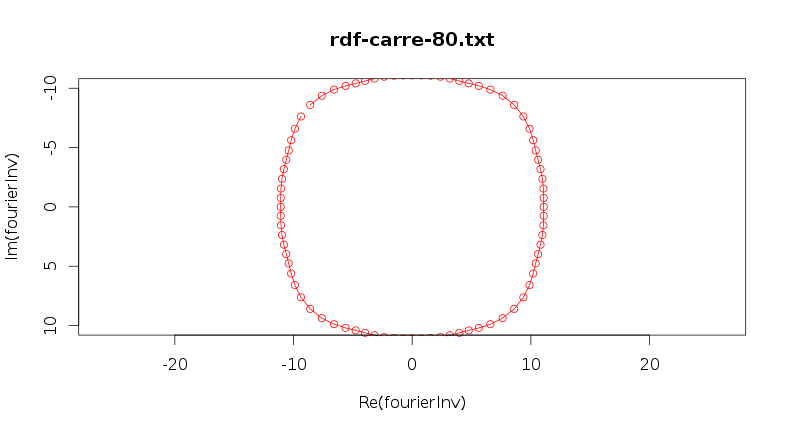
\includegraphics[width=15cm]{../resultat/carre-fourier-20.png}
      \caption{Image du carré avec 80\% des points supprimés}
    \end{figure}
  \end{center}

  \section{Réduction d'une chaîne de contour}
  Nous allons maintenant nous intéresser à l'algorithme de la corde. Cette algorithme va
  suivre les contours de la forme avec un certain nombre de point. Pour effectuer ce
  calcul, nous avons besoin de connaitre la distance des points avec la corde. Nous avons
  effectuer le calcul suivant pour trouver ces distances : 
  $abs(Im((cont - debut) * Conj(fin - debut))) / Mod(fin - debut)$.
  Cela nous a permit d'obtenir des contours plus ou moins précis en fonction du nombre
  de point.
  
  \begin{center}
    \begin{figure}[!h]
      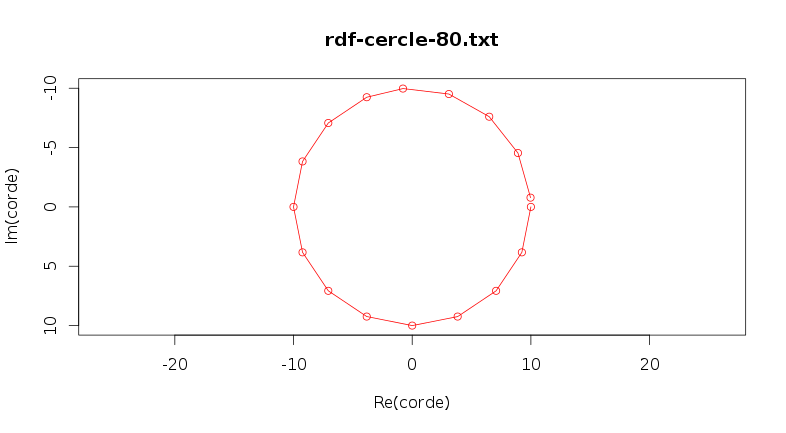
\includegraphics[width=15cm]{../resultat/cercle-corde-5.png}
      \caption{Image du cercle avec une distance maximum de 0.5 pixel}
    \end{figure}
  \end{center}
  
  \begin{center}
    \begin{figure}[!h]
      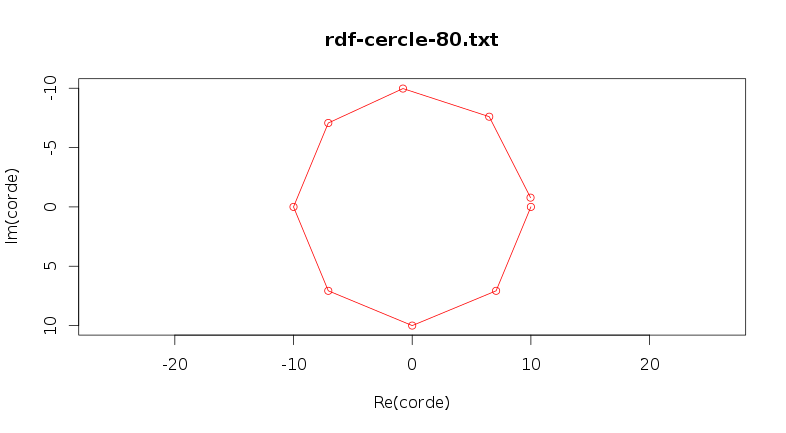
\includegraphics[width=15cm]{../resultat/cercle-corde-10.png}
      \caption{Image du cercle avec une distance maximum de 1 pixel}
    \end{figure}
  \end{center}
  
  \newpage
  
  \section{Comparaison des deux approches}
  rect :
    fourier -> 1
    corde -> 0.5 -> best (peu de point)
    
  carre :
    fourier -> 1
    corde -> 0.5 -> best (peu de point)
    
  triangle :
    fourier -> 1
    corde -> 0.8
    
\end{document}